\chapter{Vehicle Localization : The Guaranteed Estimation Problem} \label{ch:problem}
\section{Problem Formulation}
Let us denote the state of the vehicle to be tracked at time $k$ as $x_k$ and the measured state as $y_k$. The equations to predict $x_k$ from a previous step $x_{k-1}$ and the mapping from measurement, $y_k$ to state, $x_k$ is shown in equation \eqref{formula:system}, where $A$,$E$,$C$ and $F$ are known matrices, $w_k$ and $v_k$ are process noise and measurement noise at time $k$, respectively. 
\begin{equation}
\label{formula:system}
\begin{split}
x_{k+1} &= Ax_k + Ew_k\\
y_k &= Cx_k + Fv_k
\end{split}
\end{equation}

The state of the tracked vehicle can be represented using position, velocity and acceleration in x and y-direction. Different states can be estimated using different models, whereas the measured state of the vehicle is assumed to be position in x and y-direction for all models.
\begin{equation*}
y =[ 
\begin{matrix}
s_x & s_y
\end{matrix}
]^T
\end{equation*}

%The process noise($w_k$) bound is set as $[\begin{matrix}
%.1 & .1 & .4 & .4 & .1 & 0.1
%\end{matrix}]^T$ and the measurement noise($v_k$) bound is  $[\begin{matrix}
%.1 & .1
%\end{matrix}]^T$.\\

Given a model (\eqref{formula:system}), the problem of state estimation is to compute an outer bound of the state($x_k$) consisting the possible values of the true possible state of the system. The dimension of the state($x_k$), the state transition matrix($A$) and measurement matrix ($C$) differ across different models as discussed in the next section.
\section{Vehicle Model}
Three linear systems are implemented to compare the different algorithms for tracked vehicles. Although there exists highly precise vehicle models for ego vehicles, the simplest models are used here to represent the tracked vehicle since no precise model of tracked vehicles are available. In particular, physical dimensions like wheelbase or side-slip, cannot be measured directly. Another reason is that adding steering angle and yaw rate makes the system non-linear and hence does not suit all the algorithms presented. Hence, we chose to investigate the following models:
\begin{itemize}
\item \textbf{Constant Velocity Model}
\item \textbf{Constant Acceleration Model}
\item \textbf{Point Mass Model}
\end{itemize}
\subsection{Constant Velocity Model}
The vehicle is assumed to travel in constant velocity \cite{Schubert2008}. The state of the system ($x_k$), state transition matrix ($A$), and the measurement matrix($C$) is shown in \eqref{formula:cvmodel}.
\begin{equation*}
\label{formula:cvmodel}
\begin{split}
x &=
\left[\begin{matrix}
s_x & s_y & v_x & v_y
\end{matrix}\right]^{T}\\
A&= \left[\begin{matrix}
1 & 0 & \Delta T & 0\\
0 & 1 & 0 & \Delta T\\
0 & 0 & 1 & 0\\
0 & 0 & 0 & 1\\
\end{matrix}\right]\\
C&= \left[\begin{matrix}
1 & 0 & 0 & 0\\
0 & 1 & 0 & 0
\end{matrix}\right]
\end{split}
\end{equation*}
%The state transition matrix ($A$ in \eqref{formula:system}) is derived to be:\\
%$\left[\begin{matrix}
%1 & 0 & \Delta T & 0\\
%0 & 1 & 0 & \Delta T\\
%0 & 0 & 1 & 0\\
%0 & 0 & 0 & 1\\
%\end{matrix}\right]$\\
%The measurement matrix($C$ in \eqref{formula:system}) is:\\
%$\left[\begin{matrix}
%1 & 0 & 0 & 0\\
%0 & 1 & 0 & 0
%\end{matrix}\right]$\\

%\item \textbf{Singer Acceleration Model}: The acceleration of the tracked vehicle is assumed to be a first-order Markov process of the form  \cite{Singer1970}:
%\begin{equation}
%\begin{split}
%a_{k+1} & = \rho_m a_k + \sqrt{1- \rho_m^2} \sigma_m r_k\\
%\text{where}\\
%\rho_m &= e^{-\beta T}, \beta = 1/\tau_m\\
%\tau_m &= \text{target maneuver time constant}\\
%\sigma_m &= \text{target maneuver standard deviation}\\
%r_k &= \text{zero-mean unit-standard deviation Gaussian distributed random variable}\\
%T &= \text{time step}\\
%\end{split}
%\end{equation}
%The state transition matrix, $A$, measurement matrix, $C$ for each model are tabulated in Table \ref{tab:models}.
%
%\begin{table}[htbp]
%\caption{Comparison of state transition and measurement matrix for different vehicle models.\\}
%	\centering
%	\renewcommand{\arraystretch}{1.1}
%	\small	
%	\begin{tabular}{l l  l l @{}}
%		\toprule 
%		\textbf{Model} & \textbf{x} & \textbf{A} & \textbf{C} \\ \midrule
%		%-------------------------------------		
%		Constant Velocity & $\left[\begin{matrix}
%s_x \\ s_y \\ v_x \\ v_y
%\end{matrix}\right]$
% & $\left[\begin{matrix}
%1 & 0 & \Delta T & 0\\
%0 & 1 & 0 & \Delta T\\
%0 & 0 & 1 & 0\\
%0 & 0 & 0 & 1\\
%\end{matrix}\right]$
% & $\left[\begin{matrix}
%1 & 0 & 0 & 0\\
%0 & 1 & 0 & 0
%\end{matrix}\right]$\\
%Constant Acceleration & $
%\left[\begin{matrix}
%s_x \\ s_y \\ v_x \\ v_y \\a_x \\a_y
%\end{matrix}\right]$
% & $\left[\begin{matrix}
%1 & 0 & \Delta T & 0 & \frac{1}{2}\Delta T^2 & 0\\
%0 & 1 & 0 & \Delta T & 0 & \frac{1}{2}\Delta T^2 \\
%0 & 0 & 1 & 0 & \Delta T & 0\\
%0 & 0 & 0 & 1 & 0 & \Delta T\\
%0 & 0 & 0 & 0 & 1 & 0\\
%0 & 0 & 0 & 0 & 0 & 1
%\end{matrix}\right]$
% & $\left[\begin{matrix}
%1 & 0 & 0 & 0 & 0 & 0\\
%0 & 1 & 0 & 0 & 0 & 0
%\end{matrix}\right]$\\
%%Point Mass & $
%%
%%$
%%Singer Acceleration& $
%%\left[\begin{matrix}
%%s_x \\ s_y \\ v_x \\ v_y \\a_x \\a_y
%%\end{matrix}\right]$
%% & $\left[\begin{matrix}
%%1 & 0 & \Delta T & 0 & f(\Delta T)^{[\ref{eq:singermodel}]} & 0\\
%%0 & 1 & 0 & \Delta T & 0 & f(\Delta T)^{[\ref{eq:singermodel}]} \\
%%0 & 0 & 1 & 0 & g^{[\ref{eq:singermodel}]} & 0\\
%%0 & 0 & 0 & 1 & 0 & g^{[\ref{eq:singermodel}]}\\
%%0 & 0 & 0 & 0 & 1 & 0\\
%%0 & 0 & 0 & 0 & 0 & 1
%%\end{matrix}\right]$
%% & $\left[\begin{matrix}
%%1 & 0 & 0 & 0 & 0 & 0\\
%%0 & 1 & 0 & 0 & 0 & 0
%%\end{matrix}\right]$\\
%		%--------------------------------------		
%		\bottomrule
%	\end{tabular}
%	\label{tab:models}
%\end{table}
%
%\begin{equation}
%\label{eq:singermodel}
%\begin{split}
%f(\Delta T) &= \frac{1}{\beta^2}(-1+\beta\Delta T+\rho_m)\\
%g(\Delta T) &= \frac{1}{\beta} (1- \rho_m)
%\end{split}
%\end{equation}
\subsection{Constant Acceleration Model}
Although the Constant velocity Model is easy to implement, however it is dangerous to assume constant velocity. Acceleration model takes care of changing velocity and assumes constant acceleration \cite{Schubert2008}. The state of the system ($x_k$), state transition matrix ($\mathcal{A}$), and the measurement matrix($C$) is shown in \eqref{formula:camodel}.

\begin{equation*}
\label{formula:camodel}
\begin{split}
x&= \left[\begin{matrix}
s_x & s_y & v_x & v_y & a_x & a_y
\end{matrix}\right]^{T}\\
A&= \left[\begin{matrix}
1 & 0 & \Delta T & 0 & \frac{1}{2}\Delta T^2 & 0\\
0 & 1 & 0 & \Delta T & 0 & \frac{1}{2}\Delta T^2 \\
0 & 0 & 1 & 0 & \Delta T & 0\\
0 & 0 & 0 & 1 & 0 & \Delta T\\
0 & 0 & 0 & 0 & 1 & 0\\
0 & 0 & 0 & 0 & 0 & 1
\end{matrix}\right] \\
C&= \left[\begin{matrix}
1 & 0 & 0 & 0 & 0 & 0\\
0 & 1 & 0 & 0 & 0 & 0
\end{matrix}\right]
\end{split}
\end{equation*}
%$\left[\begin{matrix}
%s_x & s_y & v_x & v_y & a_x & a_y
%\end{matrix}\right]^{T}$.\\
%The state transition matrix ($A$ in \eqref{formula:system}) is derived to be:\\
%$\left[\begin{matrix}
%1 & 0 & \Delta T & 0 & \frac{1}{2}\Delta T^2 & 0\\
%0 & 1 & 0 & \Delta T & 0 & \frac{1}{2}\Delta T^2 \\
%0 & 0 & 1 & 0 & \Delta T & 0\\
%0 & 0 & 0 & 1 & 0 & \Delta T\\
%0 & 0 & 0 & 0 & 1 & 0\\
%0 & 0 & 0 & 0 & 0 & 1
%\end{matrix}\right]$.\\
%The measurement matrix($C$ in \eqref{formula:system}) is:\\
%$\left[\begin{matrix}
%1 & 0 & 0 & 0 & 0 & 0\\
%0 & 1 & 0 & 0 & 0 & 0
%\end{matrix}\right]$\\.

\subsection{Point Mass Model}
It is trivial to note that vehicles might have varying acceleration which is not satisfied in the previous models, which brings us to the Point Mass Model\cite{Althoff} which is similar to the constant acceleration model, except that the acceleration can change upto a certain limit. This model treats the tracked vehicle as a point mass, ignoring wheel-base, slip-angle etc. of the tracked vehicle. The state transition matrix and measurement matrix are same as the constant acceleration model. The acceleration bounds are set as $11.5 m/s^2$ in both x and y-direction for this paper.

\section{Zonotopes: The Set Representation}
Zonotopes are gaining fame in the set-based state estimation techniques \cite{Le2013}, due to its control of wrapping effect and that the Minkowski sum of the zonotope results in zonotopes.

Zonotopes are represented by a center, denoted by $p$ and generators, denoted by $H$. An m-zonotope in $\mathbb{R}^n$ can be defined as an affine transformation by $H$ of an m-dimensional hypercube in $\mathbb{R}^n$ centered at $p$. Minkowski sum, zonotope reduction and convex hull of zonotopes are required to be computed in the state estimation algorithms. The toolbox, CORA (COntinuous Reachability Analyzer) \cite{Althoff2018}, is used to construct zonotopes and apply the computation for zonotopes in the algorithms. 
\begin{figure}[!h]
\label{fig:zonotope}
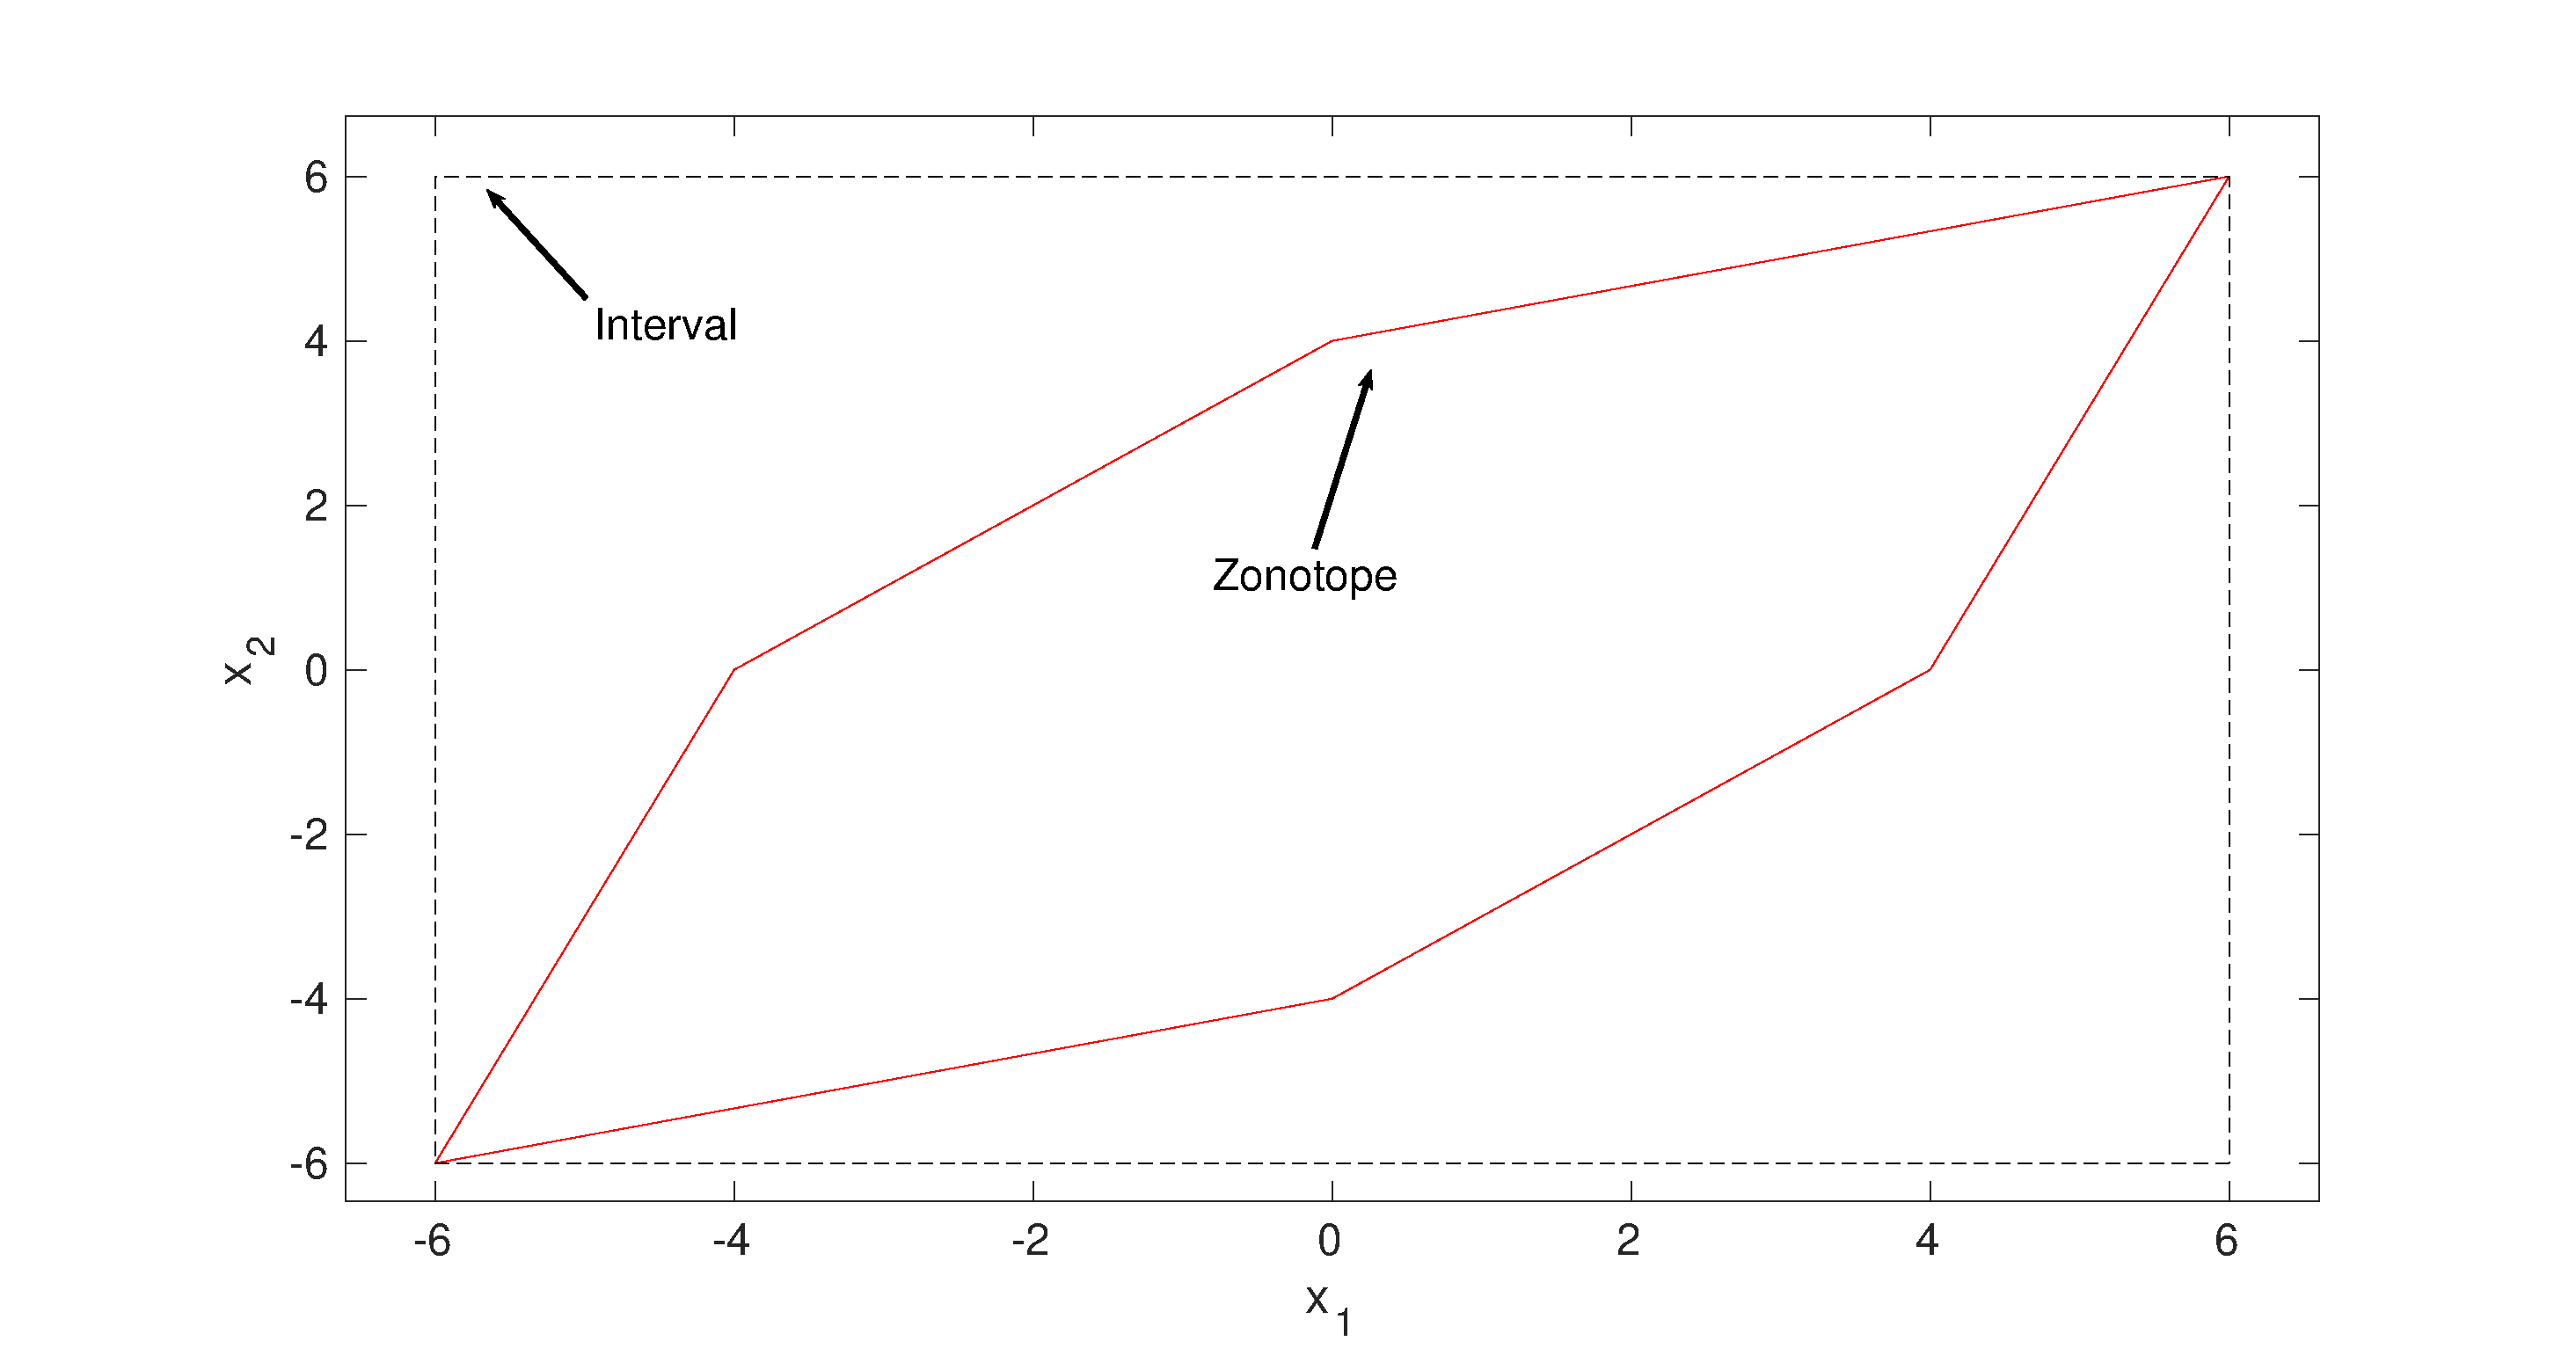
\includegraphics[scale=.25]{figures/zonotope}
\caption{An illustration of a zonotope and its interval hull in 2-D}
\end{figure}
